\documentclass{article}
\usepackage[UTF8]{ctex}
\usepackage{amsfonts}
\usepackage{amsmath}
\usepackage{float}
\usepackage{graphicx}
\usepackage{url}

\newcommand{\Bezier}{B\'ezier}%Bézier

\usepackage{color}

% paragraph
\setlength{\parindent}{0pt}
\setlength\parskip{\baselineskip}
\renewcommand{\baselinestretch}{1.2}

\begin{document}
	
	% 标题
	\title{《计算机辅助几何设计》作业}
	\author{ID号: 048  \qquad  姓名: 郑涛}  %递交作业时填上ID号和姓名
	\date{2024年11月2日}
	\maketitle
	
	
	1. Given the following cubic polynomial curve:\\
	\begin{equation*}
		P(u)=-\left(\begin{array}{c} 7/8\\5/8 \end{array}\right)u^3+
		\left(\begin{array}{c}	9\\15/4 \end{array}\right)u^2-
		\left(\begin{array}{c} 57/2\\9/2 \end{array}\right)u+
		\left(\begin{array}{c} 30\\-1 \end{array}\right)
	\end{equation*}
	1) Calculate its polar form and the vertices of its Bézier control polygon $P_0,P_1,P_2,P_3$
	within the interval[2,4], and roughly sketch this control polygon;\\
	2) Use the de Casteljau algorithm to calculate the polynomial curve at sample $u$ =
	{$\frac{5}{2}$ , 3, $\frac{7}{2}$}, and draw it in the figure in 1);\\
	3) Using the results from 2) to subdivide the curve at $u$ = 3, then subdivide the right 
	portion at its midpoint $u=\frac{7}{2}$. Draw the control polygon in the figure in 1), and 
	draw the curve $P(u)$\\
	解:\\
	\begin{figure}[H]
		\centering
		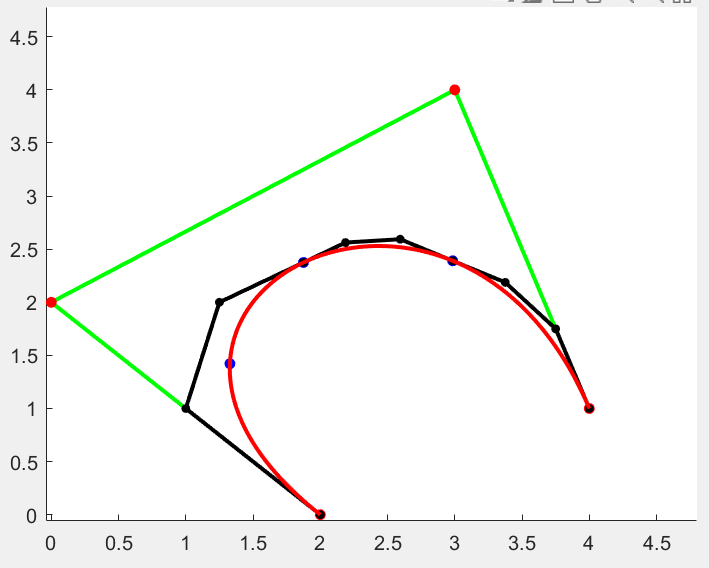
\includegraphics{1}
		\caption{}
		\label{fig:1}
	\end{figure}
	1)	
	\begin{equation*}
		f(u_1,u_2,u_3)=-\left(\begin{array}{c} 7/8\\5/8 \end{array}\right)u_1u_2u_3+
		\left(\begin{array}{c} 9\\15/4 \end{array}\right)\frac{u_1u_2+u_2u_3+u_1u_3}{3}-
		\left(\begin{array}{c} 57/2\\9/2 \end{array}\right)\frac{u_1+u_2+u_3}{3}+
		\left(\begin{array}{c} 30\\-1 \end{array}\right)
	\end{equation*}
	$P_0=f(2,2,2)=\left(\begin{array}{c} 2\\0 \end{array}\right)$,
	$P_1=f(2,2,4)=\left(\begin{array}{c} 0\\2 \end{array}\right)$\\
	$P_2=f(2,4,4)=\left(\begin{array}{c} 3\\4 \end{array}\right)$,
	$P_3=f(4,4,4)=\left(\begin{array}{c} 4\\1 \end{array}\right)$\\
	2)\\
	$u=5/2$:\\
	$$f(2,2,5/2)=3/4f(2,2,2)+1/4f(2,2,4)=\left(\begin{array}{c} 3/2\\1/2 \end{array}\right)$$
	$$f(2,5/2,4)=3/4f(2,2,4)+1/4f(2,4,4)=\left(\begin{array}{c} 3/4\\5/2 \end{array}\right)$$
	$$f(5/2,4,4)=3/4f(2,4,4)+1/4f(4,4,4)=\left(\begin{array}{c} 13/4\\13/4 \end{array}\right)$$
	$$f(2,5/2,5/2)=3/4f(2,2,5/2)+1/4f(2,5/2,4)=\left(\begin{array}{c} 21/16\\1 \end{array}\right)$$
	$$f(5/2,5/2,4)=3/4f(2,5/2,4)+1/4f(5/2,4,4)=\left(\begin{array}{c} 11/8\\43/16 \end{array}\right)$$
	$$P(5/2)=f(5/2,5/2,5/2)=3/4f(2,5/2,5/2)+1/4f(5/2,5/2,4)=\left(\begin{array}{c} 85/64\\91/64 \end{array}\right)$$
	$u=3$:\\
	$$f(2,2,3)=1/2f(2,2,2)+1/2f(2,2,4)=\left(\begin{array}{c} 1\\1 \end{array}\right)$$
	$$f(2,3,4)=1/2f(2,2,4)+1/2f(2,4,4)=\left(\begin{array}{c} 3/2\\3 \end{array}\right)$$
	$$f(3,4,4)=1/2f(2,4,4)+1/2f(4,4,4)=\left(\begin{array}{c} 7/2\\5/2 \end{array}\right)$$
	$$f(2,3,3)=1/2f(2,2,3)+1/2f(2,3,4)=\left(\begin{array}{c} 5/4\\2 \end{array}\right)$$
	$$f(3,3,4)=1/2f(2,3,4)+1/2f(3,3,4)=\left(\begin{array}{c} 5/2\\11/4 \end{array}\right)$$
	$$P(3)=f(3,3,3)=1/2f(2,3,3)+1/2f(3,3,4)=\left(\begin{array}{c} 15/8\\19/8 \end{array}\right)$$
	$u=7/2$\\
	$$f(2,2,7/2)=1/4f(2,2,2)+3/4f(2,2,4)=\left(\begin{array}{c} 1/2\\3/2 \end{array}\right)$$
	$$f(2,7/2,4)=1/4f(2,2,4)+3/4f(2,4,4)=\left(\begin{array}{c} 9/4\\7/2 \end{array}\right)$$
	$$f(7/2,4,4)=1/4f(2,4,4)+3/4f(4,4,4)=\left(\begin{array}{c} 15/4\\7/4 \end{array}\right)$$
	$$f(2,7/2,7/2)=1/4f(2,2,7/2)+3/4f(2,7/2,4)=\left(\begin{array}{c} 29/16\\3 \end{array}\right)$$
	$$f(7/2,7/2,4)=1/4f(2,7/2,4)+3/4f(7/2,4,4)=\left(\begin{array}{c} 27/8\\35/16 \end{array}\right)$$
	$$P(7/2)=f(7/2,7/2,7/2)=1/4f(2,7/2,7/2)+3/4f(7/2,7/2,4)=\left(\begin{array}{c} 191/64\\153/64\end{array}\right)$$
	3)\\
	第一段控制点:\\
	$$Q_1^{(0)}=f(2,2,2)=\left(\begin{array}{c} 2\\0 \end{array}\right),Q_1^{(1)}=f(2,2,3)=\left(\begin{array}{c} 1\\1 \end{array}\right)$$
	$$Q_1^{(2)}=f(2,3,3)=\left(\begin{array}{c} 5/4\\2 \end{array}\right),Q_1^{(3)}=f(3,3,3)=\left(\begin{array}{c} 15/8\\19/8 \end{array}\right)$$
	第二段控制点:\\
	$$Q_2^{(0)}=f(3,3,3)=\left(\begin{array}{c} 15/8\\19/8 \end{array}\right)$$
	$$Q_2^{(1)}=f(3,3,7/2)=1/4f(2,3,3)+3/4f(3,3,4)==\left(\begin{array}{c} 35/16\\41/16 \end{array}\right)$$
	$$Q_2^{(2)}=f(3,7/2,7/2)=1/2f(2,7/2,7/2)+1/2f(7/2,7/2,4)=\left(\begin{array}{c} 83/32\\83/32 \end{array}\right)$$
	$$Q_2^{(3)}=f(3,7/2,7/2)=\left(\begin{array}{c} 191/64\\153/64 \end{array}\right)$$
	第三段控制点:\\
	$$Q_3^{(0)}=f(7/2,7/2,7/2)=\left(\begin{array}{c} 191/64\\153/64 \end{array}\right),
	Q_3^{(1)}=f(7/2,7/2,4)=\left(\begin{array}{c} 27/8\\35/16 \end{array}\right)$$
	$$Q_3^{(2)}=f(7/2,4,4)=\left(\begin{array}{c} 15/4\\7/4 \end{array}\right),
	Q_3^{(3)}=f(4,4,4)=\left(\begin{array}{c} 4\\1 \end{array}\right)$$
	2.Given the following cubic polynomial curve and parameter interval [0,1]:\\
	\begin{equation*}
		F(u)=\left(\begin{array}{c}	15\\-6 \end{array}\right)u^3+
		\left(\begin{array}{c}	27\\10 \end{array}\right)u^2-
		\left(\begin{array}{c} 9\\9 \end{array}\right)u
	\end{equation*}
1) Calculate its first and second derivatives;\\
2) Calculate its polar form $f(u_1,u_2,u_3)$ and the polar forms of the derivatives $F'$ and $F''$, prove that they equal to 3$f(u_1, u_2, \hat{1})$ and 6$f(u_1, \hat{1},\hat{1})$ respectively.
Note that $f(u_1, u_2, \hat{1}) = f(u_1, u_2, 1) − f(u_1, u_2, 0)$.\\
解:\\
1)\\
$$F'(u)=\left(\begin{array}{c}	45\\-18 \end{array}\right)u^2+
\left(\begin{array}{c}	54\\20 \end{array}\right)u-
\left(\begin{array}{c} 9\\9 \end{array}\right)$$
$$F''(u)=\left(\begin{array}{c}	90\\-36 \end{array}\right)u+
\left(\begin{array}{c}	54\\20 \end{array}\right)$$
2)\\
$$f(u_1,u_2,u_3)=\left(\begin{array}{c}	15\\-6 \end{array}\right)u_1u_2u_3+
\left(\begin{array}{c}	27\\10 \end{array}\right)\frac{u_1u_2+u_2u_3+u_1u_3}{3}-
\left(\begin{array}{c} 9\\9 \end{array}\right)\frac{u_1+u_2+u_3}{3}$$
$$f'(u_1,u_2)=\left(\begin{array}{c}	45\\-18 \end{array}\right)u_1u_2+
\left(\begin{array}{c}	54\\20 \end{array}\right)\frac{u_1+u_2}{2}-
\left(\begin{array}{c} 9\\9 \end{array}\right)$$
$$f''(u_1)=\left(\begin{array}{c}	90\\-36 \end{array}\right)u_1+
\left(\begin{array}{c}	54\\20 \end{array}\right)$$
Proof:
\begin{equation*}
	\begin{aligned}
		f(u_1,u_2,\hat{1})=&f(u_1,u_2,1)-f(u_1,u_2,0)\\
		=&\left(\begin{array}{c}	15\\-6 \end{array}\right)(u_1u_2-0)+
		\left(\begin{array}{c}	27\\10 \end{array}\right)(\frac{u_1u_2+u_1+u_2}{3}-\frac{u_1u_2}{3})\\
		&-
		\left(\begin{array}{c}	9\\9 \end{array}\right)(\frac{u_1+u_2+1}{3}-\frac{u_1+u_2}{3})\\
		=&\left(\begin{array}{c}	45\\-18 \end{array}\right)\frac{u_1u_2}{3}+\left(\begin{array}{c}	54\\20 \end{array}\right)\frac{u_1+u_2}{3}-\left(\begin{array}{c}	9\\9 \end{array}\right)\frac{1}{3}\\
		=&\frac{1}{3}f'(u_1,u_2)
	\end{aligned}
\end{equation*}
\begin{equation*}
	\begin{aligned}
		f(u_1,\hat{1},\hat{1})=&f(u_1,\hat{1},1)-f(u_1,\hat{1},0)\\
		=&(f(u_1,1,1)-f(u_1,0,1))-(f(u_1,1,0)-f(u_1,0,0))\\
		=&f(u_1,1,1)-2f(u_1,1,0)+f(u_1,0,0)\\
		=&\left(\begin{array}{c}	15\\-6 \end{array}\right)(u_1-0+0)+
		\left(\begin{array}{c}	27\\10 \end{array}\right)(\frac{2u_1+1}{3}-2\cdot\frac{u_1}{3}+0)\\
		&-
		\left(\begin{array}{c}	9\\9 \end{array}\right)(\frac{u_1+2}{3}-2\cdot\frac{u_1+1}{3}+\frac{u_1}{3})\\
		=&\left(\begin{array}{c} 90\\-36 \end{array}\right)\frac{u_1}{6}+\left(\begin{array}{c}	54\\20 \end{array}\right)\frac{1}{6}\\
		=&\frac{1}{6}f''(u_1)
	\end{aligned}
\end{equation*}
	3.Given a uniform B-spline defined by the following four points and knot vector
	[0,0,1,2,3,4,5,5]:\\
	$$P_0=\left(\begin{array}{c} -2\\-10 \end{array}\right),
	P_1=\left(\begin{array}{c}	-4\\2 \end{array}\right),
	P_2=\left(\begin{array}{c}	6\\5 \end{array}\right),
	P_3=\left(\begin{array}{c}	4\\-7 \end{array}\right)$$
	1) Use the de Boor algorithm to calculate the curve position at $t$ = 2.5. Sketch the 
	control polygon and the relevant points constructed by this algorithm.\\
	2) For the B-spline in 1), calculate the corresponding Bézier control points that 
	represent the same curve. Draw the control vertices and Bézier curve in the figure 
	in 1).\\
	解:\\
	\begin{figure}[H]
		\centering
		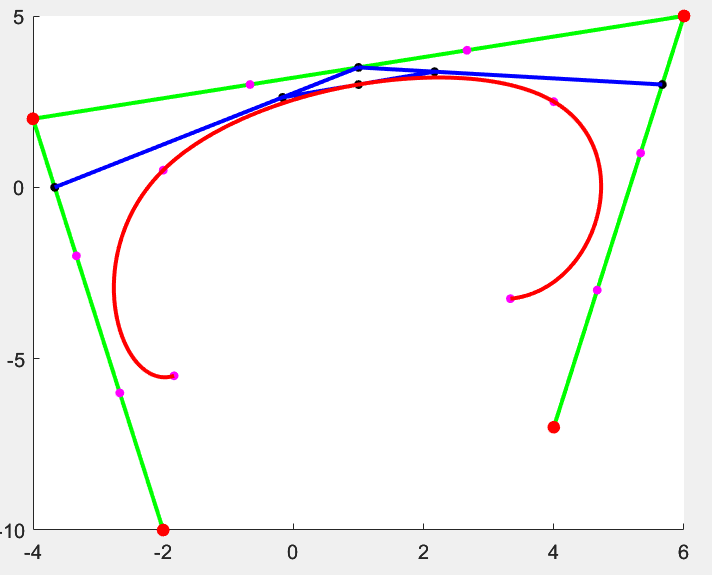
\includegraphics{3}
		\caption{}
		\label{fig:3}
	\end{figure}
	
	1)\\
	\begin{equation}\label{equ::1}
		\begin{aligned}
			x(0,1,2)=P_0=\left(\begin{array}{c} -2\\-10 \end{array}\right)\\
			x(1,2,3)=P_1=\left(\begin{array}{c}	-4\\2 \end{array}\right)\\
			x(2,3,4)=P_2=\left(\begin{array}{c}	6\\5 \end{array}\right)\\
			x(3,4,5)=P_3=\left(\begin{array}{c}	4\\-7 \end{array}\right)
		\end{aligned}
	\end{equation}
	由(\ref{equ::1}):
	\begin{equation}\label{equ::2}
		\begin{aligned}
			x(1,2,2.5)=1/6x(0,1,2)+5/6x(1,2,3)=\left(\begin{array}{c} -11/3\\0 \end{array}\right)\\
			x(2,2.5,3)=1/2x(1,2,3)+1/2x(2,3,4)=\left(\begin{array}{c}	1\\7/2 \end{array}\right)\\
			x(2.5,3,4)=5/6x(2,3,4)+1/6x(3,4,5)=\left(\begin{array}{c}	17/3\\3 \end{array}\right)\\
		\end{aligned}
	\end{equation}
	由(\ref{equ::2}):
	\begin{equation}\label{equ::3}
		\begin{aligned}
			x(2,2.5,2.5)=1/4x(1,2,2.5)+3/4x(2,2.5,3)=\left(\begin{array}{c} -1/6\\21/8 \end{array}\right)\\
			x(2.5,2.5,3)=3/4x(2,2.5,3)+1/4x(2.5,3,4)=\left(\begin{array}{c}	13/6\\27/8 \end{array}\right)\\
		\end{aligned}
	\end{equation}
	由(\ref{equ::3}):
	\begin{equation}\label{equ::4}
		\begin{aligned}
			x(2.5,2.5,2.5)=1/2x(2,2.5,2.5)+1/2x(2.5,2.5,3)=\left(\begin{array}{c} 1\\3 \end{array}\right)\\
		\end{aligned}
	\end{equation}
	2)\\
	设控制点为$Q_i(i=0,1,\dots,9)$\\
	$$\begin{aligned}
		s(t)=&\sum_{i=0}^{3}P_iN_i^m(t)\\
		=&x(0,0,1)N_{-1}^m(t)\\
		&+x(0,1,2)N_0^m(t)+x(1,2,3)N_1^m(t)+x(2,3,4)N_2^m(t)+x(3,4,5)N_3^m(t)\\
		&+x(4,5,5)N_4^m(t)
	\end{aligned}$$
	可得$$x(0,0,1)=0,x(4,5,5)=0$$
	\begin{equation}
		\begin{aligned}
			x(1,2,2)=&1/3x(0,1,2)+2/3x(1,2,3)=\left(\begin{array}{c} -10/3\\-2 \end{array}\right)\\
			x(1,1,2)=&1/2x(0,1,2)+1/2x(1,2,2)=\left(\begin{array}{c} -8/3\\-6 \end{array}\right)\\
			x(0,1,1)=&1/2x(0,0,1)+1/2x(0,1,2)=\left(\begin{array}{c} -1\\-5 \end{array}\right)\\
			x(1,1,1)=&1/2x(0,1,1)+1/2x(1,1,2)=\left(\begin{array}{c} -11/6\\-11/2 \end{array}\right)\\
			x(2,3,3)=&1/3x(1,2,3)+2/3x(2,3,4)=\left(\begin{array}{c} 8/3\\4 \end{array}\right)\\
			x(2,2,3)=&1/2x(1,2,3)+1/2x(2,3,3)=\left(\begin{array}{c} -2/3\\3 \end{array}\right)\\
			x(2,2,2)=&1/2x(1,12,2)+1/2x(2,2,3)=\left(\begin{array}{c} -2\\1/2 \end{array}\right)\\
			x(3,4,4)=&1/3x(2,3,4)+2/3x(3,4,5)=\left(\begin{array}{c} 14/3\\-3 \end{array}\right)\\
			x(3,3,4)=&1/2x(2,3,4)+1/2x(3,4,4)=\left(\begin{array}{c} 16/3\\1 \end{array}\right)\\
			x(3,3,3)=&1/2x(2,3,3)+1/2x(3,3,4)=\left(\begin{array}{c} 4\\5/2 \end{array}\right)\\
			x(4,4,5)=&1/2x(3,4,5)+1/2x(4,5,5)=\left(\begin{array}{c} 2\\-7/2 \end{array}\right)\\
			x(4,4,4)=&1/2x(3,4,4)+4/2x(4,4,5)=\left(\begin{array}{c} 10/3\\-13/4 \end{array}\right)\\
		\end{aligned}
	\end{equation}
	由于是同一条曲线,因此开花形式一样,因此对应的Bezier控制点即为:
	\begin{equation}
		\begin{aligned}
			Q_0=&x(1,1,1)=\left(\begin{array}{c} -11/6\\-11/2 \end{array}\right)\\
			Q_1=&x(1,1,2)=\left(\begin{array}{c} -8/3\\-6 \end{array}\right)\\
			Q_2=&x(1,2,2)=\left(\begin{array}{c} -10/3\\-2 \end{array}\right)\\
			Q_3=&x(2,2,2)=\left(\begin{array}{c} -2\\1/2 \end{array}\right)\\
			Q_4=&x(2,2,3)=\left(\begin{array}{c} -2/3\\3 \end{array}\right)\\
			Q_5=&x(2,3,3)=\left(\begin{array}{c} 8/3\\4 \end{array}\right)\\
			Q_6=&x(3,3,3)=\left(\begin{array}{c} 4\\5/2 \end{array}\right)\\
			Q_7=&x(3,3,4)=\left(\begin{array}{c} 16/3\\1 \end{array}\right)\\
			Q_8=&x(3,4,4)=\left(\begin{array}{c} 14/3\\-3 \end{array}\right)\\
			Q_9=&x(4,4,4)=\left(\begin{array}{c} 10/3\\-13/4 \end{array}\right)\\
		\end{aligned}
	\end{equation}
	
\end{document}











